\documentclass[]{book}

\usepackage{import}
\usepackage{preamble}

\begin{document}

\noindent BECA / Huson / 11.1 IB Math SL \hspace{2in} Name:\\*
16 November 2017
\begin{center}
{\Large Homework Review: Functions and Quadratics}\\
\textit{Complete the graphs and answer the questions.}
\end{center}

%\vspace{0.2 cm}
\subsection*{Sketching a quadratic function}
Answer on lined paper and use this sheet for the graph.

\begin{enumerate}


\item   Given $f(x)=-(x-3)^2-4$
\begin{enumerate}
    \item Write down the vertex of the function as an ordered pair.
    \item Write down the equation of the axis of symmetry.
    \item Expand the function from vertex form to standard form, $ax^2+bx+c \text{ where } a, b, c \;  \epsilon \; \mathbb{R}$.
    \item Write down the value of $f(0)$. Explain what this represents on the graph.
    \item Hence factor the function. Write down the roots.
    \item Sketch the function, labeling the intercepts with values and the vertex as an ordered pair. Show the axis of symmetry as a dotted line and label it with its equation.
\begin{figure}[!ht]
    \flushright
    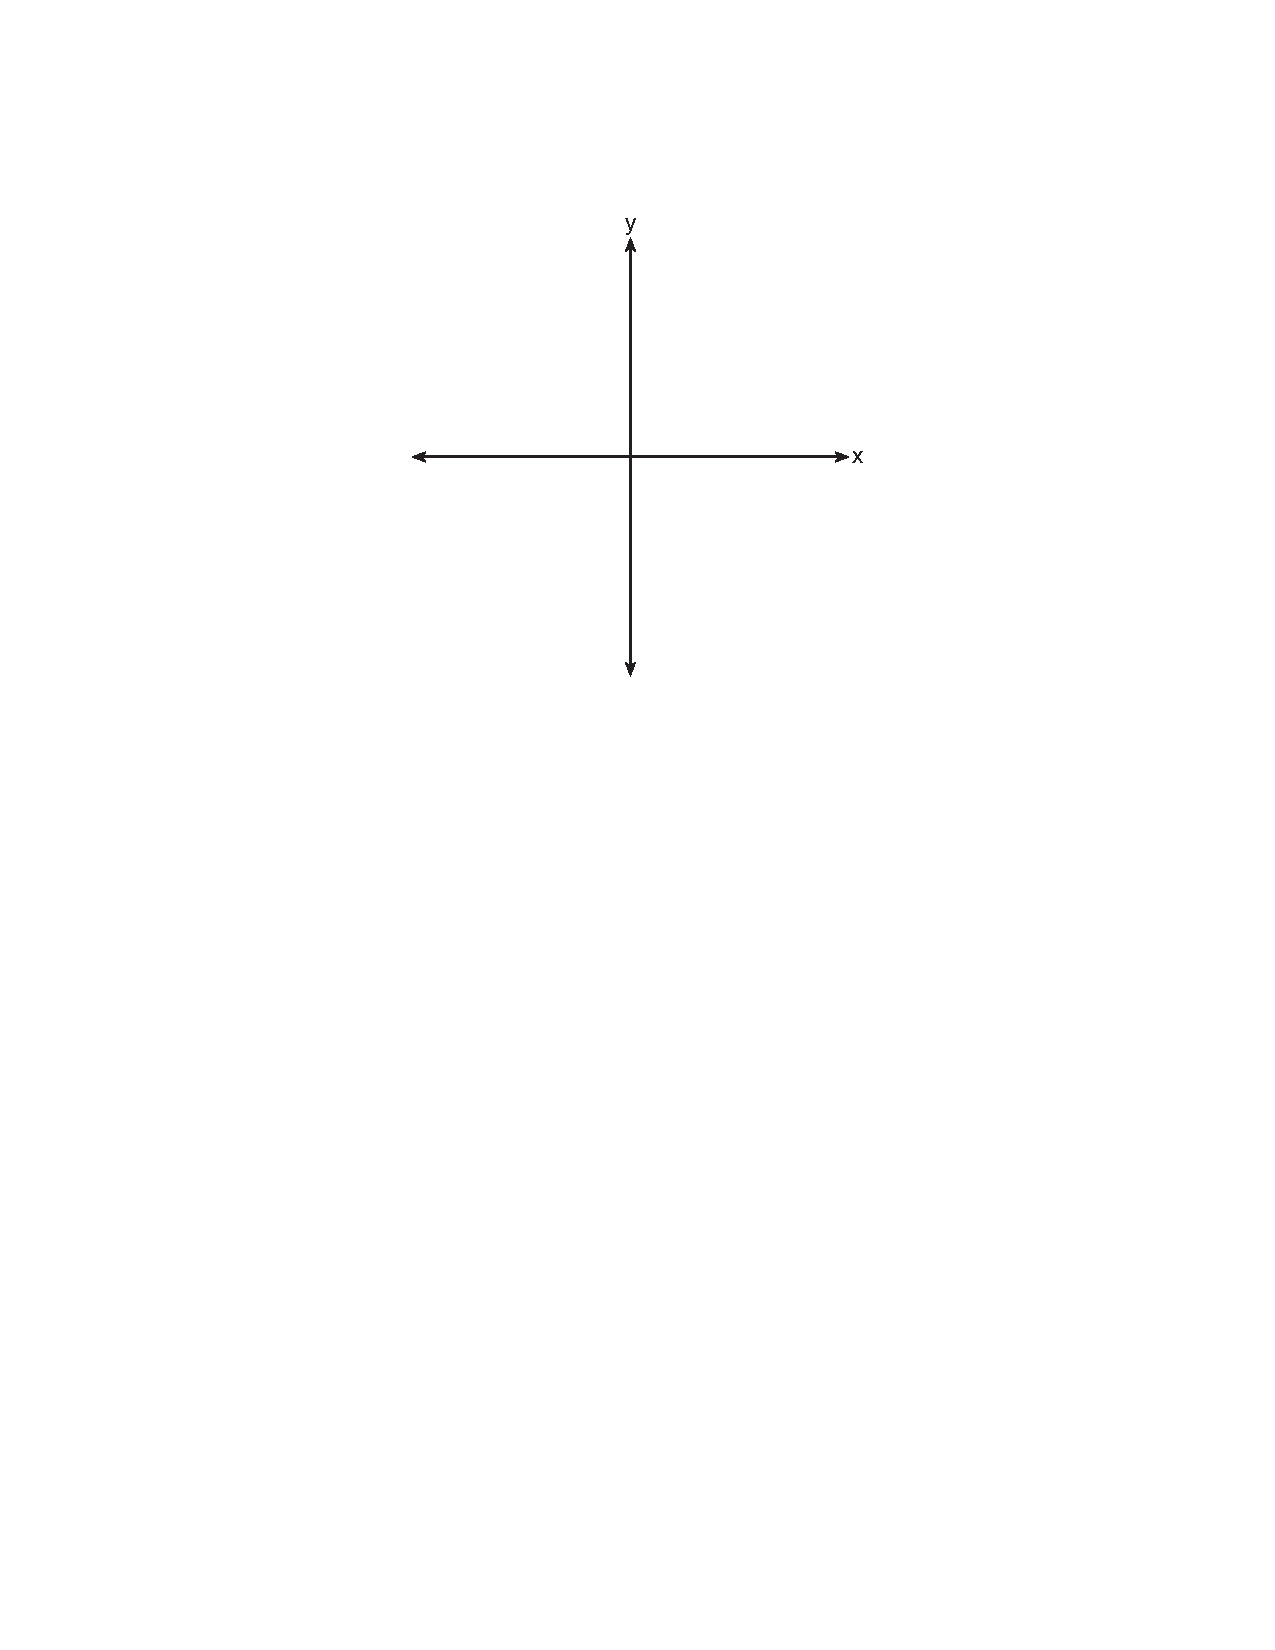
\includegraphics[width=0.6\textwidth]{simple-axes.pdf}
\end{figure}

    \item Write down the domain and range of the function.\\*[10pt]
\end{enumerate}


\newpage
\subsection*{Graphing quadratics}
Answer on lined paper. Graph the function on the grid shown below.
\item Given the function $f(x)=-x^2-2x+3$. 
\begin{enumerate}
    \item Write down the $y$-intercept.
    \item State whether the parabola opens upward or downward. Explain how you know this from the function expressed in standard form.
    \item Express the function in factored form. Hence state the solutions to $f(x)=0$.
    \item Show that the axis of symmetry of the parabola is $x=-1$.
    \item Hence state the vertex as an ordered pair. 
    \item Graph the function. Mark the vertex as an ordered pair and label each intercept with its value. Plot the axis of symmetry as a dotted line and label it with its equation.
    \item Write down the domain and range of the function.
\end{enumerate}

\begin{figure}[!ht]
    \centering
    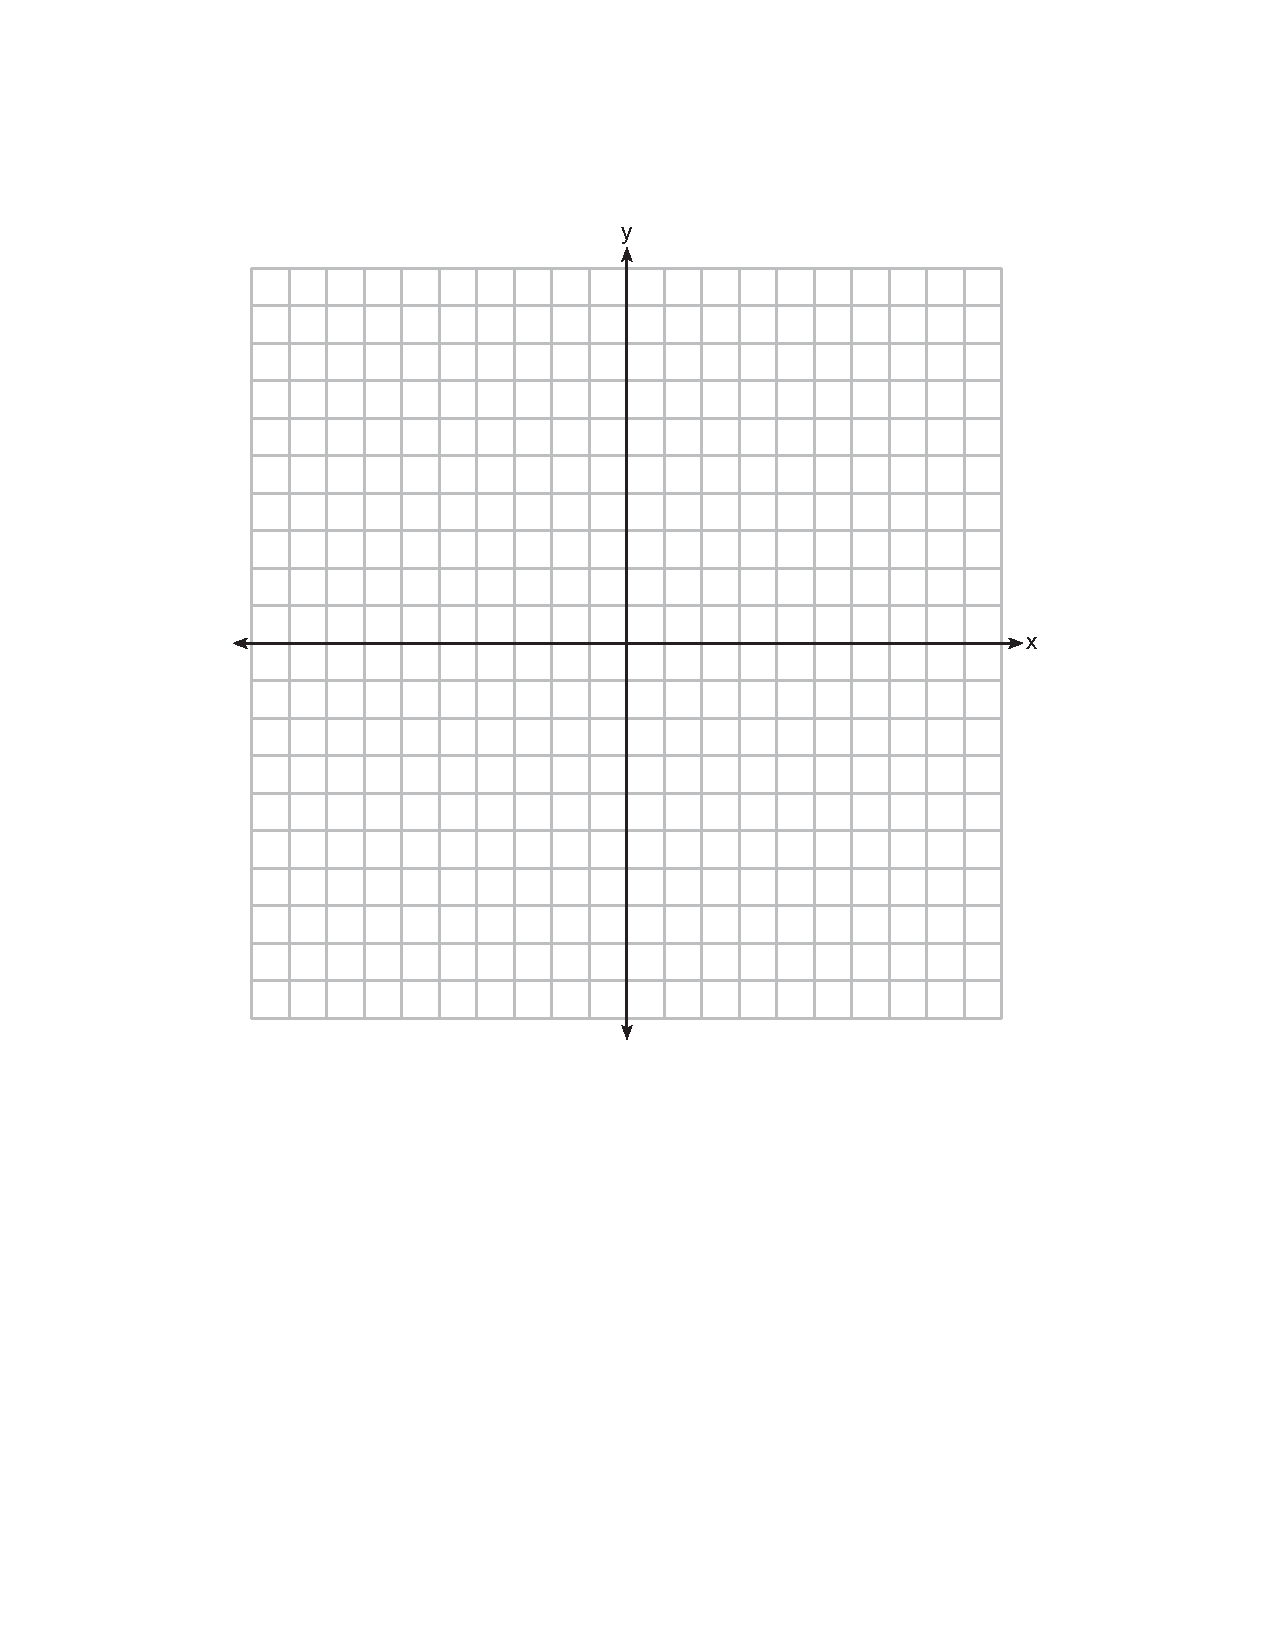
\includegraphics[width=0.75\textwidth]{regents-grid.pdf}
\end{figure}

\end{enumerate}

 \end{document}